% THIS IS SIGPROC-SP.TEX - VERSION 3.1
% WORKS WITH V3.2SP OF ACM_PROC_ARTICLE-SP.CLS
% APRIL 2009
%
% It is an example file showing how to use the 'acm_proc_article-sp.cls' V3.2SP
% LaTeX2e document class file for Conference Proceedings submissions.
% ----------------------------------------------------------------------------------------------------------------
% This .tex file (and associated .cls V3.2SP) *DOES NOT* produce:
%       1) The Permission Statement
%       2) The Conference (location) Info information
%       3) The Copyright Line with ACM data
%       4) Page numbering
% ---------------------------------------------------------------------------------------------------------------
% It is an example which *does* use the .bib file (from which the .bbl file
% is produced).
% REMEMBER HOWEVER: After having produced the .bbl file,
% and prior to final submission,
% you need to 'insert'  your .bbl file into your source .tex file so as to provide
% ONE 'self-contained' source file.
%
% Questions regarding SIGS should be sent to
% Adrienne Griscti ---> griscti@acm.org
%
% Questions/suggestions regarding the guidelines, .tex and .cls files, etc. to
% Gerald Murray ---> murray@hq.acm.org
%
% For tracking purposes - this is V3.1SP - APRIL 2009

\documentclass{acm_proc_article-sp}
%
\usepackage{url}
\usepackage{syntax}

%
\def\sharedaffiliation{%
\end{tabular}
\begin{tabular}{c}}
%
\def\eg{\textit{e.g.} }
\def\ie{\textit{i.e.} }
\def\dateparse{\texttt{DATEPARSE} }


\newcommand{\vidya}[1]{\textcolor{red}{(vidya: #1)}}
%
\begin{document}

\conferenceinfo{SIGMOD}{'16 SanFrancisco, CA USA}

\title{Does Anybody Really Know What Time It Is?\\
Automating the Extraction of Date Scalars}
\author{
% author names and affiliations
% use a multiple column layout for up to three different
% affiliations
%\author{\IEEEauthorblockN{Michael Shell}
%\IEEEauthorblockA{School of Electrical and\\Computer Engineering\\
%Georgia Institute of Technology\\
%Atlanta, Georgia 30332--0250\\
%Email: http://www.michaelshell.org/contact.html}
%\and
%\IEEEauthorblockN{Homer Simpson}
%\IEEEauthorblockA{Twentieth Century Fox\\
%Springfield, USA\\
%Email: homer@thesimpsons.com}
%\and
%\IEEEauthorblockN{James Kirk\\ and Montgomery Scott}
%\IEEEauthorblockA{Starfleet Academy\\
%San Francisco, California 96678-2391\\
%}}
\IEEEauthorblockN{The Doctor, Martha Jones, Captain Jack}
\IEEEauthorblockA{c/o Time Lords\\
The Citadel\\
Gallifrey\\
Email: \{doctor,martha,jack\}@tardis.org}\\
}


\maketitle
\begin{abstract}
With the advent of modern data visualization tools, data preparation has become a bottleneck for analytic workflows. Users who are already engaged in data analysis prefer to stay in the visualization environment for cleaning and preparation tasks whenever possible, both to preserve analytic flow and to take advantage of the visualization environment to spot inconsistent data. This has led many visualization environments to include simple data preparation functions such as scalar parsing, pattern matching and categorical binning in their analytic toolkits. One of the most common scalar parsing tasks is extracting date and time data from string representations. Several databases include date parsing ``mini-languages'' to cover the wide range of possible formats. Analysis of the usage of such functions in one visualization system shows that the parsing language syntax was difficult for users to master. 

In this paper, we present two algorithms for automatically deriving date format strings from a column of data, one based on minimum entropy and one based on natural language modeling. Both have similar accuracies of over 90\% on a large corpus of date columns extracted from an online data repository and are in substantial agreement with each other. The minimal entropy approach can also produce results below the user's perceptual threshold, making it suitable for interactive work.
\end{abstract}

%D.3.3 [Data Processing]: Data Cleaning, Natural Language Processing.
% A category with the (minimum) three required fields
\category{D.3.3}{Data Processing}{Data Cleaning, Natural Language Processing}
%A category including the fourth, optional field follows...
%\category{D.2.8}{Software Engineering}{Metrics}[complexity measures, performance measures]

\terms{Algorithms, Performance}

\section{Introduction}
In recent years, there has been a growth of interest in data visualization technologies for human-assisted data analysis using systems such as \cite{Stolte:2008,Qlik,Ahlberg:1996}. While computers can provide high-speed and high-volume data processing, humans have domain knowledge and the ability to process data in parallel, notably by using our visual systems. Most importantly, humans provide the definition of what is valuable in an analysis. Accordingly, human/computer analytic systems are essential to extracting knowledge of value to humans and their societies from the large amounts of data being generated today.


\subsection{Interactivity}
Visualization systems are most effective when they are interactive, thereby allowing a user to explore data and connect it to their domain knowledge and sense of what is important without breaking cognitive flow. In recent years, a number of such systems have been developed, both by the academic community and by the commercial sector. Exploration of data consists not only in creating visual displays, but also in creating and modifying domain-specific computations. Consequently, most data visualization systems include facilities for defining such calculations as part of the data model being analyzed. The most effective systems allow users to define these calculations as part of the analytic interaction, which permits the user to stay in the flow of analysis~\cite{Morton:2012}.

During the analytic process, a user may discover that parts of the data are not yet suitable for analysis. Solutions to this problem are often provided by data preparation tools external to the visual analysis environment, which requires the user to break their analytic flow, launch another tool and reprocess their data before returning to their analysis. If the user does not own this process (\eg it is the responsibility of another department), then there can be significant delays (including ``never.'') More subtly, the result of updated external processing may not be compatible with the user's existing work, which can lead to more time lost reconciling the new data model with the existing analysis.

From the user's perspective, the boundary between preparation and analysis is not nearly so clean cut. Bad data is often discovered using visual analysis techniques (e.g. histograms or scatter plots) and it is most natural for the user to ``clean what she sees'' instead of switching to a second tool. This leads to an ``adaptive'' process whereby users will prefer leveraging existing tools in the analytics environment (no matter how well suited to the task) over switching to another application. Thus a well-designed interactive visual analysis environment will provide tools that enable users to perform such cleaning tasks as interactively as possible.

\subsection{The Tableau Ecosystem}
In this paper, we shall be looking at an example of this problem in the context of the Tableau system. Tableau is a commercial visual analysis environment derived from the Polaris~\cite{Stolte:2008} system developed at Stanford. In addition to an interactive desktop application for creating data visualizations, the Tableau ecosystem also includes servers for publishing and sharing interactive visualizations. These servers can be privately operated by individual customers or hosted in the cloud. 

\subsubsection{Tableau Public}
Of particular relevance in the present work is a free version of the server environment called Tableau Public. Tableau Public (or ``Public'') allows authors to publish data visualizations that can be shared with the general public. The published data sets are limited to 100K rows and must be stored using the Tableau Data Engine (or ``TDE'')~\cite{Wesley:2011,Wesley:2014}, but are otherwise free to use the full analytic capabilities of the Tableau system. In particular, the TDE provides native support for all analytic calculations defined by the authoring and publishing components. Moreover, visualizations published to Public are uploaded as complete Tableau workbooks, including the data model developed as part of the analysis. This makes it a rich source of data on the analytic habits and frustrations of Tableau users.

\subsubsection{Functions}
While the existing standards for query languages are helpful for defining a core set of row-level functions, there are many useful functions beyond the standards that are only explicitly supported by a subset of RDBMSes, often with different names. And even when a database does not provide an implementation of a particular function, it is usually possible to generate it as an inline combination of existing functionality. Tableau's calculation language is designed to be a lingua franca that tames this Babel of dialects by providing a common syntax for as many of these functions as possible.

\subsection{DATEPARSE}
Among the recent additions to the Tableau function library is a function called \dateparse, the usability of which is the focus of the work in this paper.

\subsubsection{	Scalar Dates}


\begin{figure}[ht]
\centering
\includegraphics[width=\columnwidth]{figures/FigureI1}
\caption{Categorical Date Scalars.}
\label{fig:I1}
\end{figure}


The SQL-99 standard defines three temporal scalar types: \texttt{DATE}, \texttt{TIMESTAMP} and \texttt{TIME}. They are typically implemented as fixed-point types containing an offset from some epoch (\eg Julian Days.) This makes them compact to store and allows some temporal operations to be implemented very efficiently using arithmetic. Thus from the RDBMS perspective, representing dates in scalar form provides numerous benefits for users, both in terms of available operations and query performance.

Tableau models the first two of these types as ``Date'' and ``Date \& Time''; the third (pure time) is folded into Date \& Time by appending it to a fixed date of \texttt{1899-12-30}. From the analytic perspective, date types are dimensional (\ie independent variables) and can be used as either categorical (simply ordered) or quantitative (ordered with a distance metric) fields.

Categorical dates have a natural hierarchy associated with them generated by calendar binning. The visualization in Figure \ref{fig:I1} shows an example of a bar chart employing binned categorical dates in a year/quarter hierarchy.

\begin{figure}[ht]
\centering
\includegraphics[width=\columnwidth]{figures/FigureI2}
\caption{Quantitative Date Scalars.}
\label{fig:I2}
\end{figure}



Quantitative dates are typically used for time series on an axis that maps the underlying distance measure to display pixel distance. The quantitative analog to categorical binning is truncation whereby all the dates in a bin are represented by the first date in the bin. Truncation accurately preserves the distance semantics while enabling roll-up to coarser levels of detail. The visualization in Figure \ref{fig:I2} shows the same sales data in a time series rolled up to the quarter level.

These types of visualizations are difficult to specify with simple categorical string representations of dates. Thus the conversion of unparsed strings to date scalars is an important component of data modeling for analytics.


\subsubsection{Parsing}
One of the oldest data preparation problems observed in Tableau is the parsing of date scalars so that users can perform these kinds of analyses. Training materials from the early days of the company included examples of how to convert columns of integers in the form \texttt{yyyyMMdd} to date scalars. The documented solution at the time was to convert the integer to a string and perform some locale-dependent string operations before casting the string back to a date. Unfortunately, this approach had a number of problems:
\begin{itemize}
\item String operations are notoriously slow compared to scalar operations (typically 10-100x slower)
\item Default parsing of date formats is locale-dependent, and may not work when the workbook is shared across an international organization (\eg between the US and European offices)
\item The expression code was hard to understand and maintain because it used a verbose, general-purpose string-handling syntax instead of a domain language.
\end{itemize}

This is but a single format. Our studies of the workbooks on Public suggest that there are hundreds of distinct temporal date formats in user data sets. Some are common, but others can be quite idiosyncratic. Table 1 shows a selection of unusual date formats found on Public. The first example shows a time zone in the middle of the date and a year after the time; the second shows a leading unmatched bracket and a colon between the date and time components; the third shows confusion between the seconds' decimal point and the time part delimiter; the fourth shows a two digit year apostrophe on a four digit year and the fifth shows a dash separating the date and time components.



\begin{table}[ht]
\centering
%\begin{tabular}{ |l|l|l| }
\begin{tabular}{|p{0.498\linewidth}| p{0.485\linewidth}|}
\hline
\centering
\textbf{ICU Format} & \textbf{Example}\\ \hline
\scriptsize{EEE MMM dd HH:mm:ss zzz yyyy} & \scriptsize{Fri Apr 01 02:09:27 EDT 2011}\\ \hline
\scriptsize{[dd/MMM/yyyy:HH:mm:ss} & \scriptsize{[10/Aug/2014:09:30:40}\\ \hline
\scriptsize{dd-MMM-yy hh.mm.ss.SSSSSS a} & \scriptsize{01-OCT-13 01.09.00.000000 PM}\\ \hline
\scriptsize{MM ''yyyy} & \scriptsize{01 '2013}\\ \hline
\scriptsize{MM/dd/yyyy - HH:mm} & \scriptsize{04/09/2014 - 23:47}\\ \hline
\end{tabular}
\label{tab:dateformats}
\caption{Unusual Date Formats.}
\end{table}


Our first solution to this problem was to add a new function to the Tableau calculation language called \dateparse. This function would take a string column and convert it to a datetime using a special purpose domain language for describing dates. Such functions exist in a number of databases (\eg Oracle, Postgres and MySQL) and adding it to the TDE was straightforward, so it was a natural addition to the function library.

We chose the date parsing syntax defined by the International Components for Unicode (or ICU) project~\cite{ICU} for the common domain language because it mirrored what was available in the Tableau code base, and translating this syntax into the formats used by various database vendors (\eg MySQL, Oracle, Postgres) was relatively painless. There are a few patches of non-overlapping functionality, but they tend to be obscure and we provide warnings when functionality is missing.

\subsubsection{	Usability}
After shipping this new function to our user base, we investigated how it was being applied in the field. We examined a few months of workbooks that had been uploaded to Public after the release to see if and how it was being used. We found that although there were a number of new calculations using \dateparse, the error rate for the domain language syntax was about 15\%. \dateparse was capable of solving the problem, and some users were able to discover it, but the syntax did not appear to be easy to use reliably.

\subsection{Automated Format Extraction}
One solution might have been to design a graphical environment that enabled users to construct valid patterns. This would have involved a substantial development investment with no guarantee that the result would be correct if the user misunderstood the environment. Instead, we have developed two algorithms for automating the derivation of the format string, each of which uses a different machine learning technique. Both algorithms result in over 90\% parsing accuracy -- and 100\% syntactic correctness because they are machine generated.

% vidya: this probably should be its own section
% hawkfish: Not sure it is big enough, but I can see the logic.

\subsection{Related Work}

Data preparation has been a known analytic bottleneck since at least the description of the Potter's Wheel system~\cite{Ramen:2001}. Since then, several other interactive data preparation systems have been proposed, including Data Wrangler~\cite{Kandel:2001} and Google Refine~\cite{refine}. While effective, these systems all make assumptions about possible date formats (\eg the domain system in~\cite{Ramen:2001}), which we suggest are too restrictive for real world data.

The Minimum Descriptive Length technique was first proposed in Rissanen~\cite{Rissanen:1978}.  We have built on the version described in~\cite{Ramen:2001}.

Related work on parsing languages, outlier detection.

\subsection{Overview}
The rest of this paper is organized as follows: The next section introduces the parameters of the problem space. The following two sections describe the two different algorithms, one using Minimum Descriptive Length and the other using Natural Language Processing. In section 5, we evaluate the algorithms on a corpus of 30K columns, both by sampling the outputs manually and then by using the algorithms to validate each other. We then discuss future work in section 6 and conclude in section 7.


\section{Parameters}
Before delving into detailed descriptions of the two algorithms, we describe the common elements of the problem they are intended to solve. These are the input data, the output language and the interpretation of the output language for partial dates.

\subsection{Input Data}
The training data and test data are taken from data sets published to a free, online data analysis website. The published data includes both the raw data and how it was used for analysis. The service limits data sets to a maximum of 100K rows stored in a database which supports an implementation of \dateparse.  We selected a large number of string columns whose names suggested that they might contain temporal data. We included words from multiple languages besides English and extracted the column's locale (actually the collation) along with the data.

\subsubsection{NULL Filtering}
Each column was then reduced to a maximum sample set of 32. We excluded domain values that appeared to be representations of \texttt{NULL}:
\begin{itemize}
\item Values containing the substring \texttt{NULL}
\item Values containing no digits and at most one non-whitespace character (\eg \texttt{" / / "})
\item Values on a list of empirically determined common \texttt{NULL} values (\eg \texttt{0000-00-00}, \texttt{NaN})
\end{itemize}
Columns that had no remaining valid samples were discarded. 

\subsubsection{Sampling}
The remaining samples were hashed and sorted on the hash value, with the top 32 values being retained as the column's sample. We can increase the sample size if needed, but for dates, it appears to be an adequate number. In any case, the median number of non-null rows per domain in our test data is 50, so increasing the sample size would have little benefit.

\subsubsection{Numeric Timestamps}
After NULL filtering, there remained one common class of date representation that was unsuited for parsing via our date format syntax, namely numeric timestamps. This included Unix epoch timestamps (expressed as second, millisecond or microsecond counts from \texttt{1970-01-01}) and Microsoft Excel timestamps (expressed fractional days since \texttt{1900-01-01}). A simple test to check that the column was numeric and inside a specific range of values representing recent dates allowed us to tag these columns to avoid analyzing them further (and incidentally to identify them for generating a simple date extraction calculation for the user.)

\subsection{The ICU Date Format Language}
The date format syntax we selected is the one provided by the ICU open-source project. We chose it because we were already using ICU in the code base, we had access to the source code, and it provides localized date part data for a large number of languages.

The syntax is documented at the ICU web site~\cite{ICU}. While fairly complete, it has a few limitations that we ran into when evaluating the algorithms:
\begin{itemize}
\item No support for 4 letter year abbreviations (\eg \texttt{Sept.})
\item No support for ordinal days (\eg \texttt{July 4th})
\item No support for quarter postfix notation (\eg \texttt{2Q})
\item No support for variant meridian markers (\eg \texttt{a.m.})
\end{itemize}

These limitations did not affect the results significantly, and in the future we hope to submit ICU extensions to handle some of these issues.

One other quirk of the ICU syntax may be a contributing factor to the user confusion around writing correct ICU date formats. The use of lexicographical case in the meta-symbols of the format language can be confusing (\eg \texttt{y} is used for years, but \texttt{M} is used for months while \texttt{m} is used for minutes.) Another advantage of an automated algorithm is that it hides such problems from most users, significantly improving the usability of the function.

\subsection{Partial Dates}
Many of the date formats that we encountered were incomplete dates, which necessitated creating rules for what date scalar they represented.

ICU's date parsing APIs allow the specification of default values for parts when a format does not contain them. In our implementation, all time fields are set to \texttt{0} (midnight) and the date fields are set based on whether the format contains any date part specifications. When date parts are present, we use \texttt{2000-01-01} as the set of default date parts as it is the start of a leap year. When dealing with pure time formats, we model the output as a date/time and use \texttt{1899-12-30} for the date parts.

ICU will also parse Time Zones (which the algorithms recognize but the visualization system does not model) and Quarters (which we interpret as the first month of the period.) RDBMSes such as Oracle and Postgres that support time zones will be able to take advantage of  identified time zone fields.


\section{Minimal Descriptive Length}
The first algorithm is a Minimum Descriptive Length \cite{mdl} approach derived from the domain system presented in \cite{PottersWheel}. We describe a number of extensions to their structure extraction system to support more complex redundancy, non-English locales, improved performance and date-specific pruning.

\subsection{Domains}
\cite{PottersWheel} presents an algorithm for deriving a common structure for a set of strings by breaking each string down into a sequence of domains. These domains are described by an interface that includes:
\begin{itemize}
\item A required inclusion function to test for membership in the domain (\texttt{match})
\item An optional function to compute the number of values in the domain with a given length (\texttt{cardinality})
\item An optional function to update statistics for the domain based on a given value (\texttt{updateStatistics})
\item An optional function to prevent consideration of a domain that is redundant (\texttt{isRedundantAfter}).
\end{itemize}

In our approach, we implement all of these functions, but with significant changes to the last one, which we will describe below.

With this interface, we can now define a set of domains for each date part that we wish to be able to parse. These are mostly straightforward enumerations and numeric ranges, each tagged with the ICU format code. Since the ICU parser is flexible about parsing single or double digit formats, we use double-digit formats, but accept one or two digits. One important exception to this rule is for years, which are fixed width fields (2 or 4).

We also included some enumerated domains for handling constant strings and some simple regular expression domains for delimiters such as spaces, punctuation or alphabetic characters. We found that the inclusion of arbitrary numeric domains caused the run time to grow exponentially as the number of possible matches could not be pruned intelligently. This restriction extends to domains that can contain arbitrary digit sequences (such as any). Because of this restriction, the algorithm cannot extract non-date numeric fields.

\subsection{Redundancy Extensions}
A difficulty in using this kind of structure extraction is that the algorithm for enumerating structures is exponential in the number of domains. This is especially true in the date format problem because there are identical domains (e.g. months and meridian hours), nearly identical domains (e.g. days and hours) and there are often no field delimiters (e.g. \texttt{2012Mar06134427}). To handle this, we have extended the existing pruning API with two other sets of domain identifiers:
\begin{itemize}
\item A set of \textit{prunable} identifiers, which are not allowed to precede the domain. For example, once we have a month field, no other month fields should be generated. Each month domain therefore lists all the month domains in its prunable set.
\item A set of \textit{context} identifiers, one of which must have been previously generated before the domain is considered. For example, a meridian domain can only be generated once an hour field has been found, but there may be other intervening fields.
\end{itemize}

\subsection{Performance}
Structure enumeration is computationally expensive, so we added a number of enhancements to the original domain extraction algorithm to keep the run time low enough for interactivity.

\subsubsection{Domain Characteristics}
Date domains typically have small widths, so we found it advantageous to provide the shortest and longest match sizes for use in structure enumeration and matching.

Date domains are also often uniform in that adding more characters to a mismatch will not help. For example, a 2-digit day domain that does not match a 1-letter substring will not be able to generate a match by adding more characters.

\subsubsection{Parallel Evaluation}
We have also identified two opportunities for parallel computation during structure enumeration.

The first computationally expensive operation is the enumeration of structures for a given sample. To parallelize this step, each thread is given a subset of the samples and independently produces a set of candidate domains. When all threads have completed, the duplicates are removed to produce a single list of candidate structures.

The second computationally expensive operation is the evaluation of each generated structure over the entire sample set. This includes computation of the MDL, recording of domain statistics and parameterizing the structure. These tasks are simple to parallelize, because there are no overlaps between the data for each structure.

\subsection{Unparameterization}
Domain parameterization is an important part of generating compact representations via MDL, but it creates problems for date recognition. For example, if a set of dates contains a constant month string (e.g. all values are in September) it is important to keep track of the month name domain. Consequently, when we parameterize a constant generic <Word> domain, we tag it with the date part domain that it matches (if any). We then need to apply an additional pruning step to remove any structures that also found an equivalent domain (e.g. two-digit month). These rules are equivalent to the context-based redundancy rules above, but have to be applied again after parameterization of generics.

\subsection{Global Pruning}
The pruning rules used for the structure extraction reduce the search space dramatically, but they are also contextual and can only look backwards. The domains also contain a fair amount of ambiguity that requires the application of domain knowledge. We therefore found it necessary to add some post-generation global pruning rules:
\begin{itemize}
\item The set of date parts cannot contain place value gaps (e.g. structures that have year and day without month are removed.)
\item Similarly, the set of time parts cannot contain place value gaps and must also be in place value order (times are never written in orders such as \texttt{mhs}.)
\item The existence of time parts cannot make dates incomplete (e.g. patterns like year-day-hour are removed.)
\item Two digit years require special handling. In particular, they cannot appear adjacent to a two-digit field if the structure contains punctuation. (This can come up in some small early 21st century year domains where a two-digit year can masquerade as almost any numeric field.)
\end{itemize}

These global pruning rules are simple and intuitive, but are essential to further reducing the search space.

\subsection{Locale Sensitivity}
Providing an acceptable international user experience requires correctly handling the locale of the column text. Accordingly, at the start of the structure extraction we use the column locale to create a set of domains containing locale-sensitive strings such as month names. We also use the locale to map these strings to upper- and lower-case in addition to the ICU mixed case strings. This enables us to accurately compute MDL statistics without having to map the candidate strings at runtime (which would be slow).

Knowing the locale of a string is not always helpful. In our data set, we found numerous cases where the locale was specified (e.g. Sweden) but the data was actually in English. Accordingly, we test both locales and rank the combined results.
Tableau currently does not support non-Gregorian calendars. Therefore, we have built this system for the Gregorian calendar only. ICU does support non-Gregorian calendars and we expect this system could be applied to them as well.

\subsection{Ranking}
MDL structure analysis naturally produces a ranked list of format candidates, but we have found that a number of other properties of the formats should be preferred over simple compactness:
\begin{itemize}
\item Since we have a set of samples, we can apply the candidate format to the strings to see how well it performs. Formats with fewer parse errors are preferred.
\item Date parts can be considered a place-value system, so we prefer "more significant" components (e.g. month-day-year over hour-minute-second).
\item If two formats from different locales give the same results, prefer the original column locale. The sample set may have missed an example where this could be important.
\item If the format has an ambiguous date order (e.g. all days are less than 12), then prefer the default date order of the locale. Again, the sample set may have missed a counterexample, so this is the best option.
\item Once these semantic preferences have been considered, we then prefer the more compact (MDL) representation.
The output of the algorithm is now an ordered list of formats and associated locales. These can then be used to drive a user interface that allows the user to choose between the possibilities or the top-ranking format can simply be used automatically.
\end{itemize}

\section{Natural Language Processing}
(motivate why an NLP approach was considered. Also add technical detail on programming environment and parser used for grammar)

\subsection{Context-Free Grammar}
ICU date-time formats are well defined both structurally and semantically, and can be defined by a context-free grammar (CFG). A CFG is commonly defined as a set of productions or rules of the form A ? ? where A is a variable, ? is a sequence of variables and terminal symbols (the tokens that make up the alphabet of the language) plus null (? ), and the production symbol (?) indicates that the variable A can be expanded into ? . A CFG can be formally specified with four components: V, T, P, and S, where V is the set of variables, T the set of terminal symbols, P the set of productions, and S the set of available start symbols (a non-empty subset of V) [cite]. 

While there are several functionally equivalent notations for representing CFG, we use the \textit{Backus-Naur Form} (BNF) for defining the grammar rules for \dateparse formats. In particular, we use the \textit{Extended Backus-Naur Form} (EBNF) as the notation is more compact and readable for frequently used constructions~\cite{Grune:1990}. 

We define a grammar for identifying date-time strings based on other EBNF based date-time formats [cite] as a reference. A partial definition of the grammar is found below (see supplementary material for complete definition):

\begin{grammar}
<TimeGrammar> ::= <Hours> ':' <Minutes> ':' <Seconds> ;\\

<DateGrammar> ::= <BigEndianDate> 
				\alt <MiddleEndianDate> 
				\alt <LittleEndianDate>;

<DateTimeGrammar>  ::= <DateGrammar> 
					\alt <TimeGrammar>;
					

<BigEndianDate> ::= <Year> <Month>  <Day> ;

<MiddleEndianDate> ::= <Month> <Day> <Year>;

<LittleEndianDate> ::= <Day> <Month> <Year>;

<Year> ::= <TwoYear> | <FourYear>;

<Month>  ::= <MonthFullForm> | <MonthAbbrForm> | <MonthLetterForm> | <MonthNumber>;

<Day>     ::= d d (between 01 and 28-31, depending on month/year);

<Hour> ::= <TwelveHour> | <TwentyFourHour>

<TwelveHour> ::= d d (between 00-12);

<TwentyFourHour> ::= d d (between 00 and 23);

<d> ::= `0' | `1' | `2' | `3' | `4' | `5' | `6' | `7' | `8' | `9'

\end{grammar}



\subsection{Translation to ICU Format}

\subsection{Production Rule Constraints and Variants}

The EBNF date-time grammar includes a large number of syntactically correct but semantically invalid
date-time expressions. While we have added range restrictions to symbols such as \texttt{Hour} (1--12 for 12-hour format and 1--24 for 24-hour format), \texttt{Days} (1--7), \texttt{Month} (1--12), there are special cases that need to be accounted for. For example, there is no  `November 31, 2015', `February 29, 2013', or `Sunday, May  5, 1965'. November only as 30 days in any year; 2013 was not a leap year; and May 5, 1965 was a Wednesday.

While custom production rules can be added to the existing grammar to exclude such expressions, this approach is not optimal as it leads to a rather large grammar that needs to account for every single semantically valid date-time sequence of terminal symbols. Rather, we modify the existing grammar with the following additional constraints to the \texttt{Day} terminal symbol for excluding such expressions:

\begin{itemize}
\item Restriction on the distribution of $30$ and $31$:
Months usually alternate between lengths of 30 and 31 days. We can use x mod 2 to get an alternating pattern of 1 and 0, then just add our constant base number of days:

\begin{equation}
\texttt{Day} = 30 + x \Mod 2
\end{equation}

where $x \in [1..12]$ for each of the $12$ months.

Except February, Equation $1$ addresses January and March through July. After July, the pattern should skip one, and the rest of the months should follow the alternating pattern inversely.

To obtain an inverse pattern of alternating 0 and 1, we add 1 to the dividend:

\begin{equation}
\texttt{Day} = 30 + (x + 1) \Mod 2
\end{equation}

In Equation $2$ the number of days for August through December is correct ($x \in [8..12]$), but not for the remaining months. We hence introduce a bit-masking function so that the equation is equal to 1 over the desired domain and 0 otherwise. Multiplying a term by this expression will result in the term being cancelled out outside its domain. To mask the latter piece of our function, we need an expression equal to $1$ where $8 \le x\le 12$. Floor division by 8 works well, since $x < 16$.

Now if we substitute this expression in the x + 1 dividend of Equation $2$, we can invert the pattern using our mask:

\begin{equation}
\texttt{Day} = 30 + (x + \floor{\frac{x}{8}}) \Mod 2
\end{equation}


\item LeapYear Restriction for February:
While the above restriction applies to all months barring February, we also apply a constraint to the number of days for February, based on whether the year is leap year or not. For this, we define a new symbol in the grammar called \texttt{LeapYear}. If an expression containing the month `February' or any such variant (\textit{e.g.} `Feb', `2') with the day `29' and a year, would need to resolve the \texttt{Year} symbol to be a \texttt{LeapYear}, defined as:

\begin{equation}
\texttt{Year} \Mod 4 == 0
\end{equation}

\end{itemize}

Equations $3$ and $4$ are now added as constraints to the \texttt{Days} symbol in the grammar.

\subsection{Probabilistic Context-Free Grammar}
Pattern-recognition problems such as parsing date and time formats initiate from observations generated by some structured stochastic process. In other words, even if the initial higher-level production rule of the grammar is known (i.e. date, time or date-time), there could be several directions that the parser resolves to. For example, in a date string \texttt{5/6/2015}, the pattern could either be \texttt{M/d/yyyy} or \texttt{d/M/yyyy}. 

In the context of CFGs, probabilities have been used to define a probability distribution over a set of parse trees defined by the CFG, and are a useful method for modeling such ambiguity~\cite{Collins:2003,Manning:1999}. The resulting formalism called Probabilistic Context-Free Grammar (PCFG), extends the CFG by assigning probabilities to the production rules of the grammar. During the process of parsing the date-time pattern, the probabilities are used as a filtering mechanism to rank the pattern(s) that a given string resolves to in the grammar. The parser then chooses the parse tree with the maximum probability.

(add the rules for how probabilistic weights are assigned to the CFG)

\subsection{Extensions to PCFG}

\subsubsection{Columnar Context}
Once we have created a PCFG model of a process, we can apply existing PCFG parsing algorithms to identify a variety of date-time formats. However, the parser's success is often limited in the types of the dominant patterns that it can identify. In addition, the standard parsing techniques generally require specification of a complete observation sequence. In many contexts, we may have only a partial sequence available (\textit{e.g.} an incomplete entry). Finally, we may be interested in computing the probabilities of date-time patterns that the grammar may not explicitly define. To extend the forms of evidence, inferences, and pattern distributions supported, we need a flexible and expressive representation for the distribution of structures generated by the grammar. We adopt Bayesian networks for this purpose, and define an algorithm to generate a probabilistic distribution of possible parse trees corresponding to a set of date-time patterns as opposed to individual ones. 


\subsubsection{Locale and File Name Context}

%�	Explain why we use a probabilistic version of the grammar
%�	Explain how the production rules are created based on the ICU format
%�	Extensions to the parser to account for columnar context for maximizing the probabilistic occurrence of the dominant pattern
%�	Other semantic extensions � looking at the file name, adding rules for leap year, using external dictionaries for non-English terms


\section{Testing}
%1 what are the questions to answer
%2 setup (machine/code implementation/data) could be one setup per experiment or as a whole if they are identical
%3. how to perform the experiments
%4. what are the observed results
%5. what are the conclusions(discussions) from the results.

For each of the two algorithms described, we want to measure the fraction of candidate date columns that the algorithm is able to recognize. We describe a large training and experimental corpus that we collected, followed by the results of applying each algorithm to that data.
 
\subsection{Data Preparation}

The training data and test data are taken from data sets published to a free, online data analysis website. This website contains data sets that users analyzed and were interested in sharing with other people through the web. It may not be representative of data in other settings such as corporate data warehouses, but each data set is one that a user was willing to invest some time in analyzing. The published data includes both the raw data and how it was used for analysis. The service limits data sets to a maximum of 100K rows stored in a columnar database with collated strings.

We collected the contents of columns with names containing any of the following strings: Date, month, created, dt (abbreviation for date), mes (month in Spanish), datum (date in German), fecha (date in Spanish), data (date in Portuguese), and the day character used in Chinese and Japanese. Roughly 95\% of the data on the website is in English, but we attempted to include non-English data that was available. Fields of any data type other than date or datetime were analyzed, including strings, integers, and floats. One file containing the unique non-null values was created for each scanned column, and the column collation was stored in a second table.

Most database and spreadsheet systems already detect a limited set of date formats. For instance, typing the string \texttt{"12/31/1999"} into Microsoft Excel, is automatically interpreted as the date \texttt{1999-12-31}. The Microsoft Jet library \vidya{need a reference here} used to read these text files detects a few date formats as well. Any column already converted by Excel or Jet was not included in this study.

The data was divided into two sets, one for training and one for validation. There were 30,968 files in the training set and 31,546 files in the resulting verification set.

% Should we quantify the number of formats excluded here?

\subsubsection{NULL Filtering}
Each column was then reduced to a maximum sample set of 32. We excluded domain values that appeared to be representations of \texttt{NULL}:
\begin{itemize}
\item Values containing the substring \texttt{NULL}
\item Values containing no digits and at most one non-whitespace character (\eg \texttt{" / / "})
\item Values on a list of empirically determined common \texttt{NULL} values (\eg \texttt{0000-00-00}, \texttt{NaN})
\end{itemize}
Columns that had no remaining valid samples were discarded. 

\subsubsection{Sampling}
The remaining samples were hashed and sorted on the hash value, with the top $32$ values being retained as the column's sample. We can increase the sample size if needed, but for dates, it appears to be an adequate number. In any case, the median number of non-null rows per domain in our test data is $50$, so increasing the sample size would have little benefit.

\subsubsection{Numeric Timestamps}
After NULL filtering, a common class of date representation (numeric timestamps) remained that was unsuited for parsing via our date format syntax. This included Unix epoch timestamps (expressed as second, millisecond or microsecond counts from \texttt{1970-01-01}) and Microsoft Excel timestamps (expressed fractional days since \texttt{1900-01-01}). A simple test to check that the column was numeric and inside a specific range of values representing recent dates allowed us to tag these columns to avoid analyzing them further (and incidentally to identify them for generating a simple date extraction calculation for the user.)


\subsubsection{Partial Dates}
Many of the date formats that we encountered were incomplete dates, which necessitated creating rules for what date scalar they represented.

ICU's date parsing APIs allow the specification of default values for parts when a format does not contain them. In our implementation, all time fields are set to \texttt{0} (midnight) and the date fields are set based on whether the format contains any date part specifications. When date parts are present, we use \texttt{2000-01-01} as the set of default date parts as it is the start of a leap year. When dealing with pure time formats, we model the output as a date/time and use \texttt{1899-12-30} for the date parts.

ICU will also parse Time Zones (which the algorithms recognize but the visualization system does not model) and Quarters (which we interpret as the first month of the period.) RDBMSes such as Oracle and Postgres that support time zones will be able to take advantage of  identified time zone fields.

\subsection{Evaluation}
Once the training data was analyzed, it was grouped by date format. A sample of each produced date format was manually labeled. This allowed us to quickly skip over very common formats like \texttt{MM/dd/yyyy} and focus our efforts on much less common formats. The samples were judged as to whether the produced format was reasonable and were tagged with correct formats if the produced format was unreasonable.

Further manual tagging focused on the files most likely to represent dates. Many of the files in the collection are not actually dates, such as fields named ``updated by'' (which contain ``date''). A random sample of 850 columns named exactly ``date'', ``time'' or ``month'' (case-insensitive) were manually judged.\\

\subsubsection{Minimum Descriptive Length}
Testing of the MDL algorithm was performed on a 24-core Dell T7610 running Windows 7 with the data stored on a 250GB SSD.

\begin{table}[ht]
\centering
\bgroup
\def\arraystretch{1.5}
\begin{tabular}{|p{0.48\linewidth}| p{0.24\linewidth}|}
\hline
\textbf{Number of Records} & 31,546\\ \hline
\textbf{Error Rate} & 27.95\% \\ \hline
\textbf{Analysis Speed ($\mu s$)} & 2,245.04 \\ \hline
\textbf{Validation Speed ($\mu s$)} & 1.65 \\ \hline
\textbf{Median Not Null} & 50 \\ \hline
\end{tabular}
\egroup
\label{tab:mdlstats}
\caption{MDL Parsing Statistics.}
\end{table}

To test the MDL algorithm, we ran it over the set of samples from each validation file to generate a ranked list of formats for the file. Each format was then applied to the entire file's data set, recording both the number of errors and the elapsed times. In cases where we generated multiple formats and the main format produced errors, we applied the second format to the unparsed strings. The summary statistics from this processing are presented in Table 2.

The analysis speed is the average time needed per sample for structure extraction. At 2.5ms, this is well below most human perceptual thresholds for a set of 32 samples, so any latency in command execution would be restricted to the ability of the underlying database to provide the samples for analysis in a timely manner. (As a column store, the database can often supply such domains without a full table scan, further improving responsiveness.) 

The validation speed is the average time needed to parse a value, and provides an estimate of how fast the ICU implementation can process string values into scalars and works out to 620K values per core per second.\\
 
\begin{figure}[ht]
\centering
\includegraphics[width=\columnwidth]{figures/FigureM2}
\caption{MDL Error Rate}
\label{fig:M2}
\end{figure}


The error rate reflects the fact that only about 40\% of the files have an associated format that parses the non-null values without error. To examine the error rate in greater detail, we turn now to Figure \ref{fig:M2}.

On the left hand side, we can see that the algorithm found 744 distinct formats that parsed 13,424 files with no error. This is a remarkable number of valid formats and underscores the need for this kind of algorithm. Raising the error rate threshold to 5\% results in about 2500 formats found in 15,000 files, or nearly half of the files. 

What do these formats look like? Figure \ref{fig:M3} shows a histogram of the 25 most common formats containing a year format code at the 5\% threshold, color-coded by error rate. (A sample value is provided to the right of each bar for illustrative purposes.) The formats have also been filtered to files with at least 5 samples. Most of the samples are clearly dates with a wide range of formats (the format where the time zone is between the time and the year is surprisingly common.)
 
\begin{figure}[ht]
\centering
\includegraphics[width=\columnwidth]{figures/FigureM3}
\caption{MDL Output}
\label{fig:M3}
\end{figure}


Some of the dates are clearly just numbers, but our approach is to assume that when the user tells us that the column contains dates we should find the best fit. The samples include dates from a wide range of historical sources (\eg Roman pottery dates) so we have elected to defer the date identification task to the user.

\subsubsection{Natural Language Processing}


We implemented the grammar, training and parsing in Python 3.4.1 using the Natural Language Toolkit libraries~\cite{nltk} on a quad core Dell T7600 running Windows 7. The complexity of the CYK parsing algorithm is $O(n^{3}|G|)$, where $n$ is the length of the input and $|G|$ is the size of the grammar~\cite{Younger67}. The PCFG grammar uses a set of $22$ phrase-level non-terminals and $30$ terminals to classify the various constituents in the corpus. Because the CYK algorithm finds the maximum likelihood solution, there are no search errors (rather probability $p = 0$, and a modification in the grammar is required to improve accuracy.

Similar to the MDL algorithm described in the previous subsection, the CYK parser is run over the same set of samples from each validation file to generate a ranked list of parse trees representing the date-time formats. As a second pass of the parser, starting from the most probable parse tree, each parse tree is then applied to the entire file's columnar data to determine the dominant pattern(s). For the second pass, we can parallelize the CYK parsing because the dependencies between reapplying the ranked list of parse trees are very sparse.

The initial average parsing speed to compute the ranked set of probable parse trees is $0.93s$, while the average time taken to compute the overall dominant pattern(s) for the entire column of data is $1.4s$. While the natural language parsing implementation is in Python as the NLTK package is easily configurable, we could expect greater speed-up in parsing performance by employing C/C++ CYK parsing libraries.


Out of the $31,546$ files used for testing, the NLP parser identified a dominant format for $26, 534 (84.11\%)$ where $p >= 0.5$. $1634$ unique formats were identified. Figure \ref{fig:NLP1} shows a histogram of the most common formats identified containing \texttt{Year}. There are some variations compared to Figure \ref{fig:M3} including the fact that we are not filtering the results by any error rate in the NLP parsed results.

\begin{figure}[ht]
\centering
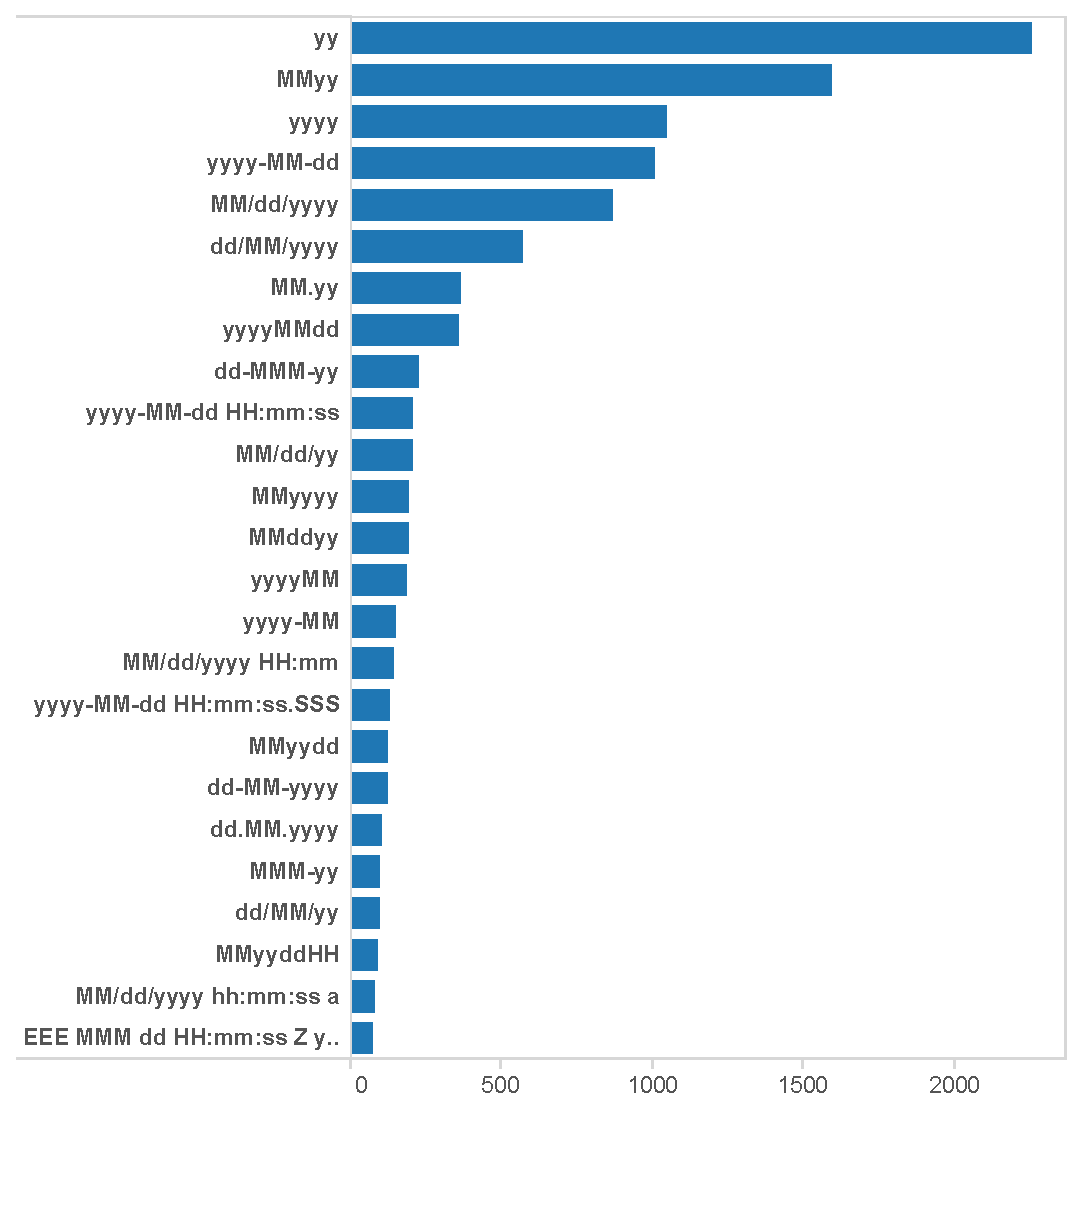
\includegraphics[width=\columnwidth]{figures/FigureNLP1}
\caption{Most common date formats identified by the NLP algorithm.}
\label{fig:NLP1}
\end{figure}

\subsubsection{Cross-Checking}
We compared the results of the minimum description length and natural language processing algorithms. The two algorithms match for 97.9\% of our validation set. The main differences in the results are due to small differences in the implementations. The minimum description length implementation recognizes formats with leading plus and minus signs, but these are almost certainly numbers, not dates. The minimum description length implementation also recognizes the Excel date formats, but this was not supported by the natural language implementation. There was one file that contained formats such as \texttt{`Fall 2000'} and \texttt{`Spring 2000'}, and the two algorithms picked different seasons in their format. One other file contained a set of integers that are not actually dates, and one algorithm picked \texttt{MMyyyy} format, while the other picked \texttt{HHmmss} format.

\subsubsection{Production}

Although both algorithms achieved comparable high accuracies in parsing date time strings, we utilized the minimum description length method in the production code of our system. This was primarily due to the fact that the MDL algorithm was written in C++, allowing for higher performance. We believe that NLP version if written in C++ as opposed to Python, would lead to better performance. 

\section{Future Work}
While we are satisfied with the results so far, we found a number of columns that we were not able to process with these techniques. Many columns contained multiple date formats, and we would like to recognize this situation and generate predicate-based calculations to increase the accuracy of the results and thereby make the experience even more seamless for the user. Other columns contain date ranges, which we would like to handle by generating multiple calculations, possibly by combining regular expressions with date parsing.

In this paper, we have only considered the parsing of strings, but dates are often formatted as integers (\textit{e.g.} \texttt{201507016}). It is significantly faster to decompose integers into date parts using arithmetic operations (\textit{e.g.} \texttt{mod} and \texttt{div}) than by using slower, locale-sensitive string parsing functions. Moreover, the number of possible formats is low enough that we may be able to enumerate them. Timestamp preparation from numeric representations is another form of preparation which we would like to automate.

In the course of our research, we have also identified a number of date part variants (\textit{e.g.} ordinal dates, four-letter month abbreviations, alternate meridian markers and postfix quarter syntax) that we would like to commend to the ICU project and maybe provide implementations of.


\section{Conclusion}
In this paper, we have described two effective algorithms for extracting date format strings from a small set of samples, one using a minimum descriptive length approach and one using natural language techniques. Both algorithms are accurate enough to be used automatically without user involvement. The MDL algorithm is also fast enough to deploy in an interactive environment.

While validating the algorithms on a large corpus, we also found that the number of distinct formats in the wild is surprisingly high, and demonstrates the wisdom of including general-purpose date parsing functions in data visualization tools, data cleaning tools and RDBMSes. In particular, it is interesting to note that the most prominent open source RDBMSes (\eg MySQL and Postgres) both have a built-in version of \texttt{DATEPARSE}, possibly reflecting that this is a common need that gets implemented when users are empowered to extend the function library of an RDBMS.


%ACKNOWLEDGMENTS are optional
\section{Acknowledgments}
We would like to thank to Douglas Adams for encouraging this work; BBC Wales for providing the resources to productize it; and Doctor Who Live, whose harrowing live demonstration of episode production in front of several thousand people inspired this project.


%
% The following two commands are all you need in the
% initial runs of your .tex file to
% produce the bibliography for the citations in your paper.
\bibliographystyle{abbrv}
\bibliography{dateparse}  % sigproc.bib is the name of the Bibliography in this case
% You must have a proper ``.bib'' file
%  and remember to run:
% latex bibtex latex latex
% to resolve all references
%
% ACM needs 'a single self-contained file'!
%

\balancecolumns
% That's all folks!
\end{document}
